\documentclass{article}
\usepackage[utf8]{inputenc}
\usepackage{amsmath, amssymb, amsthm}
\usepackage{float}
\usepackage[shortlabels]{enumitem}
\usepackage{graphicx} % Required for inserting images
\title{MATH512 - Project 4}
\author{Wasif Ahmed, Haoxiang Deng, Jacob Fein-Ashley, Kanav Malhotra, Longzhe Yang}
\date{April 2024}

\begin{document}

\maketitle

\section*{Question 1}

Refer to Figure~\ref{fig:convergence1}

\begin{figure}[H]
    \centering
    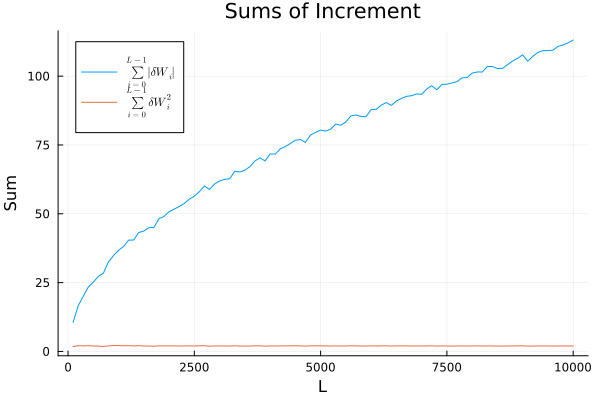
\includegraphics[scale=0.6]{imgs/convergence1.png}
    \caption{Stochastic Plots}
    \label{fig:convergence1}
\end{figure}

Notice that as the $L$ parameter increases, the $|\delta W_i|$ term is unbounded while $\delta W_i^2$ converges to $2$ in probability.

\section*{Question 2}

\begin{enumerate}
    \item 
        \begin{figure}[H]
            \centering
            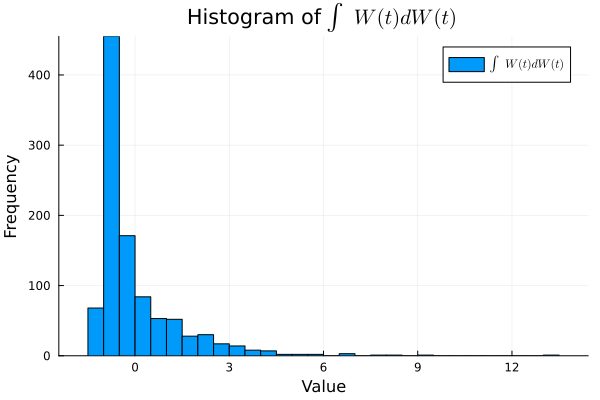
\includegraphics[scale=0.6]{imgs/2a.png}
            \caption{2a}
            \label{fig:2a}
        \end{figure}

    \item 
        \begin{figure}[H]
            \centering
            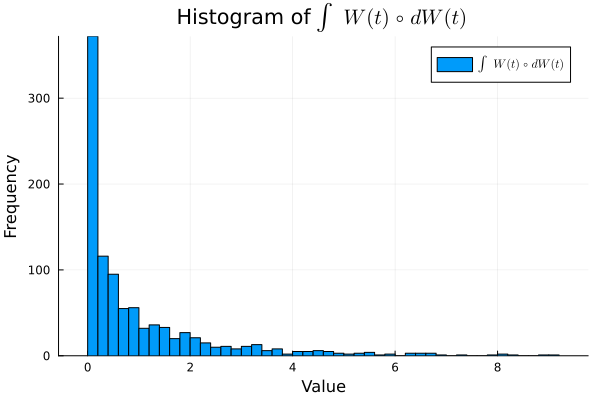
\includegraphics[scale=0.6]{imgs/2b.png}
            \caption{2b}
            \label{fig:2b}
        \end{figure}
    \item
        \begin{figure}[H]
            \centering
            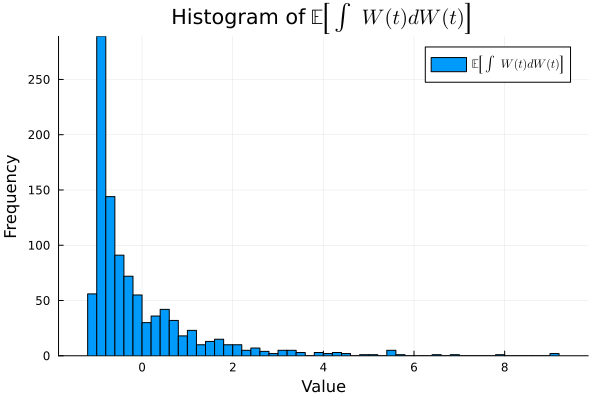
\includegraphics[scale=0.6]{imgs/2c.png}
            \caption{2c}
            \label{fig:2c}
        \end{figure}
    \item
        \begin{figure}[H]
            \centering
            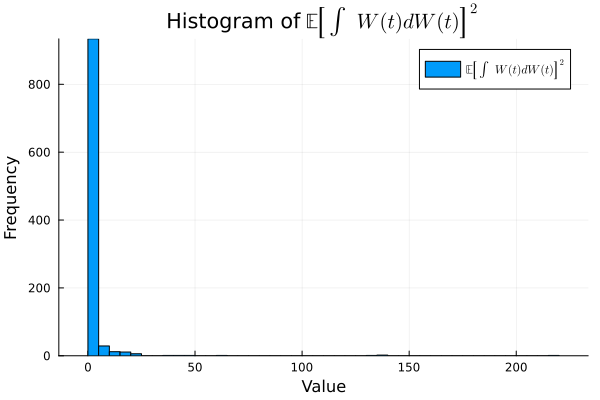
\includegraphics[scale=0.6]{imgs/2d.png}
            \caption{2d}
            \label{fig:2d}
        \end{figure}
    \item
        \begin{figure}[H]
            \centering
            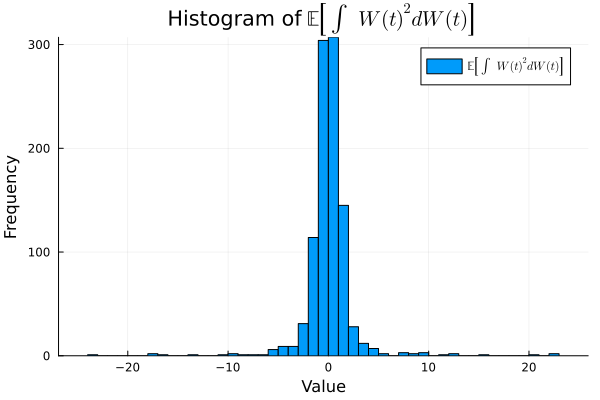
\includegraphics[scale=0.6]{imgs/2e.png}
            \caption{2e}
            \label{fig:2e}
        \end{figure}

    \item 
        \begin{figure}[H]
            \centering
            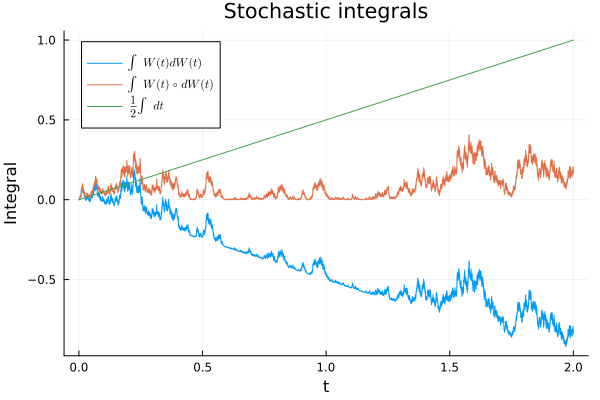
\includegraphics[scale=0.6]{imgs/2f.png}
            \caption{2f}
            \label{fig:2f}
        \end{figure}
\end{enumerate}

\section*{Question 3}

\section*{Question 4}
\begin{figure}[H]
    \centering
    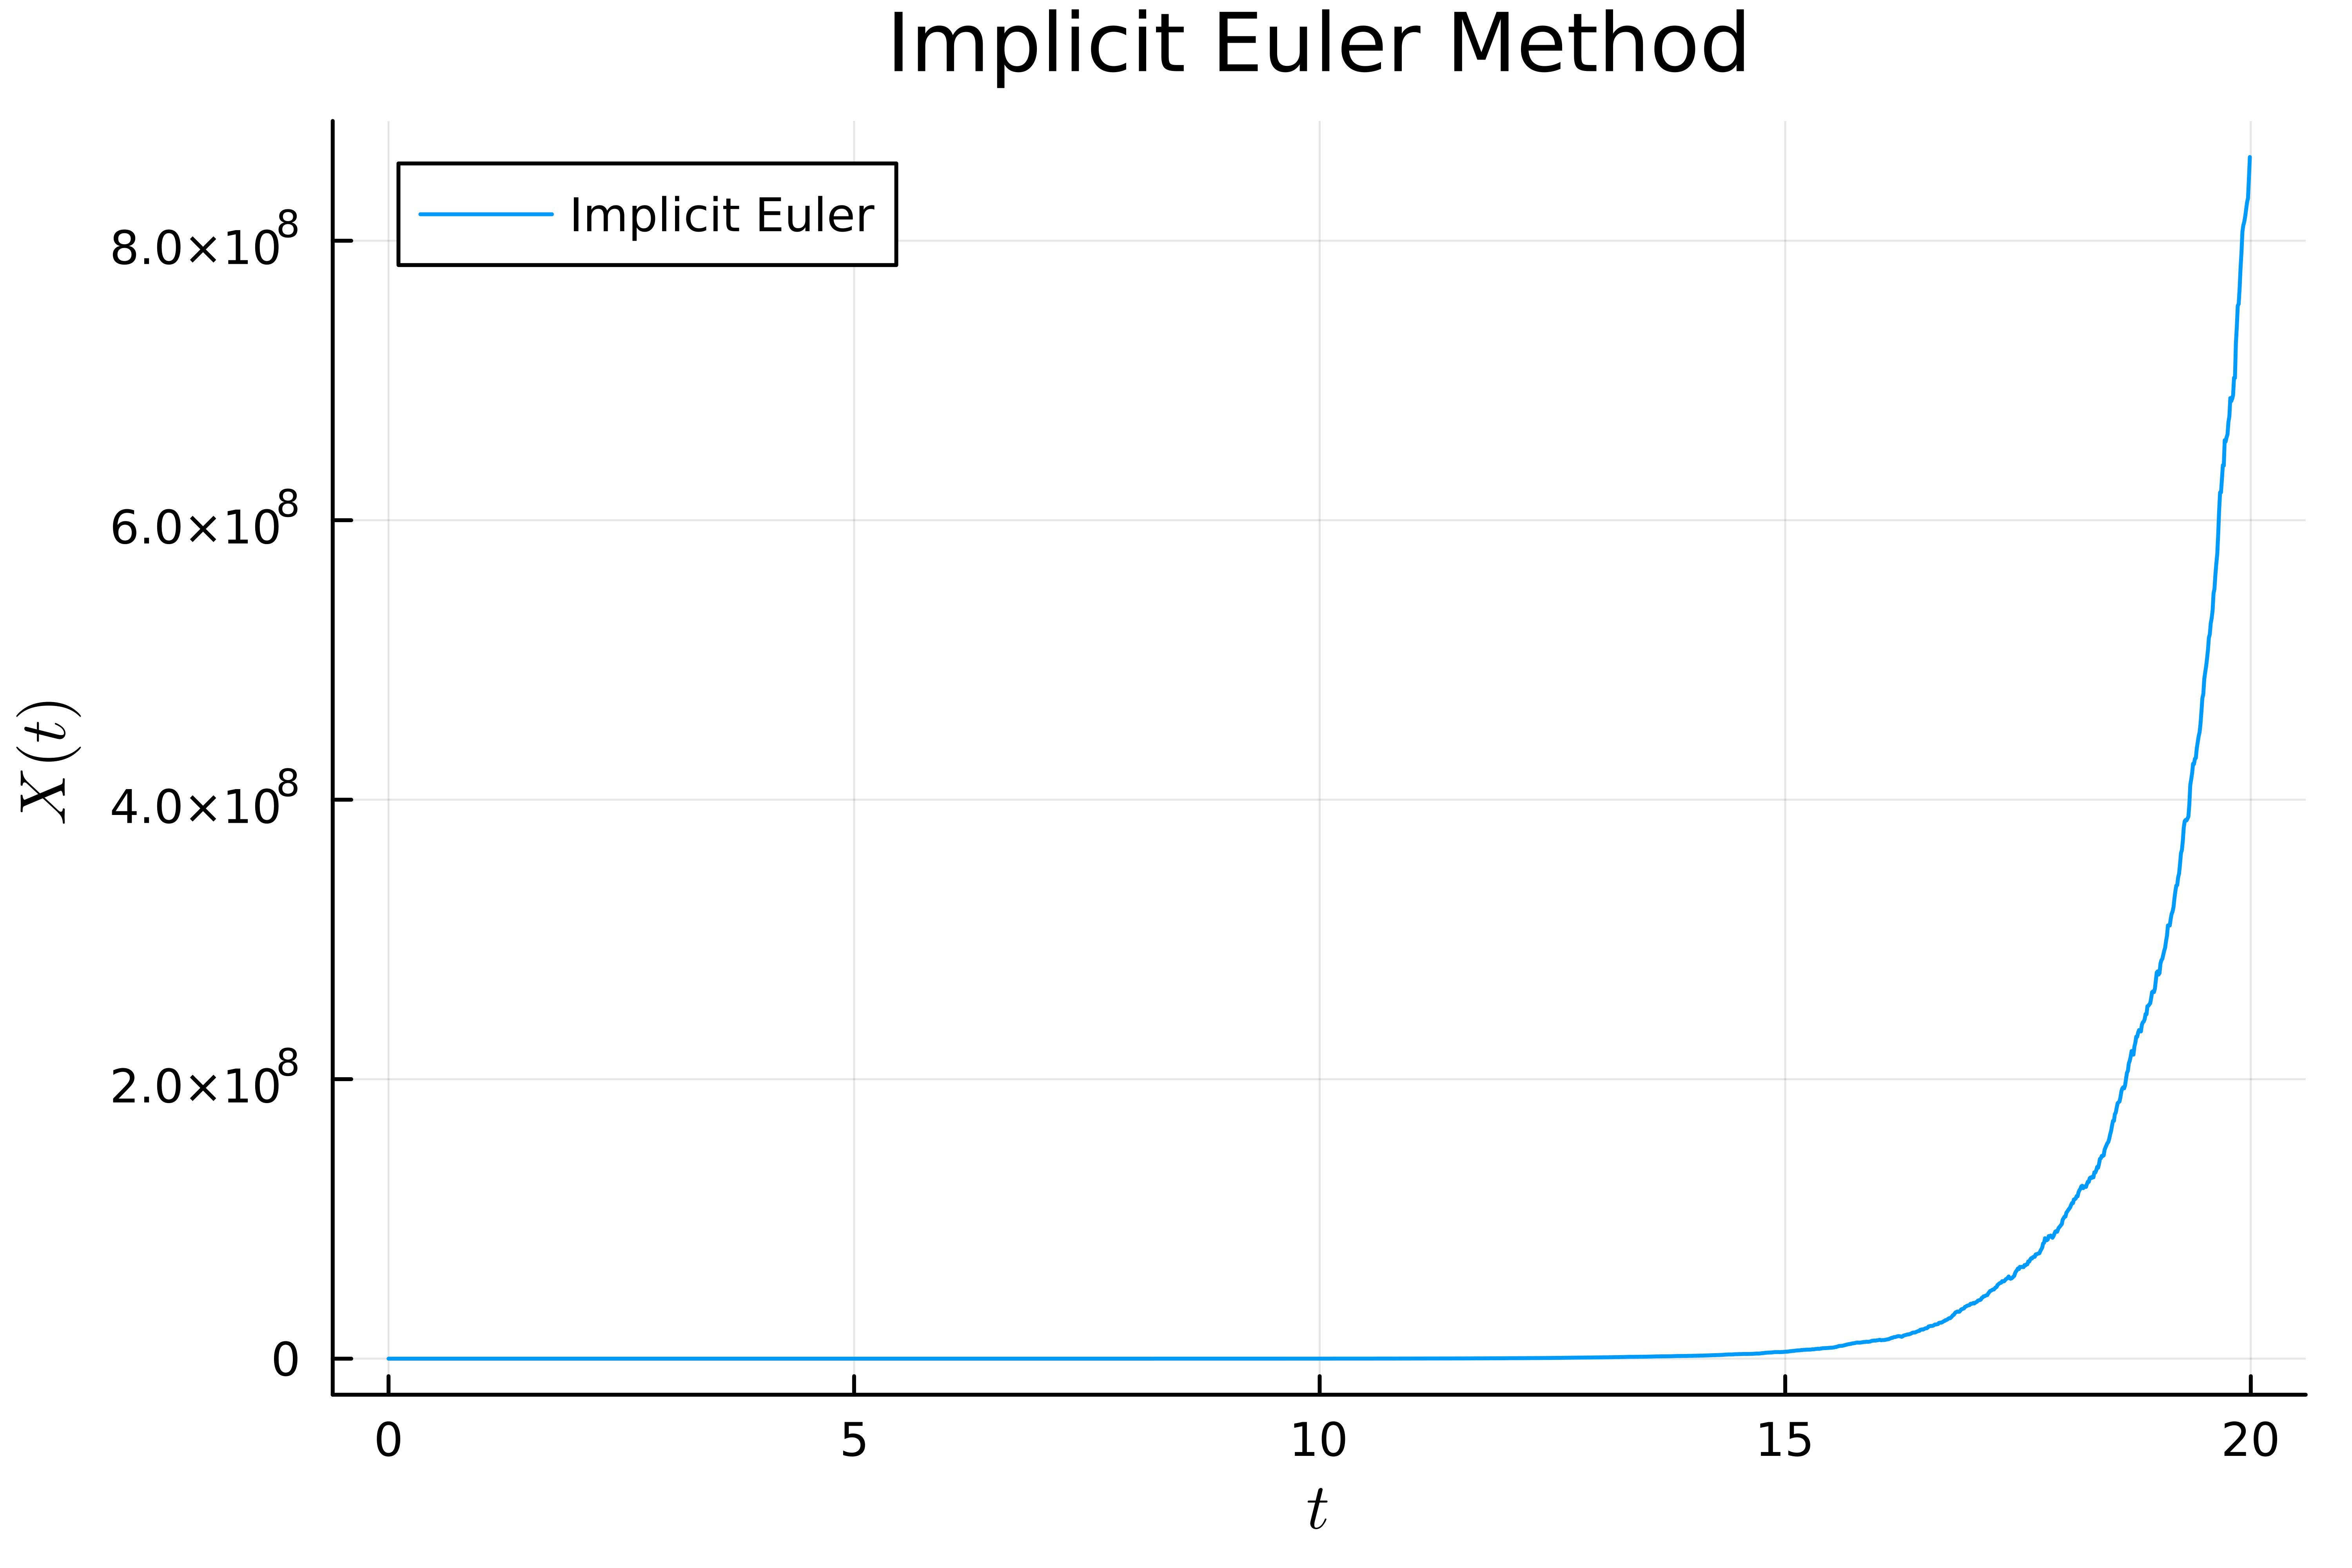
\includegraphics[scale=0.05]{imgs/4implicit_euler.png}
    \caption{Implicit Euler}
    \label{fig:impliciteuler}
\end{figure}

\begin{figure}[H]
    \centering
    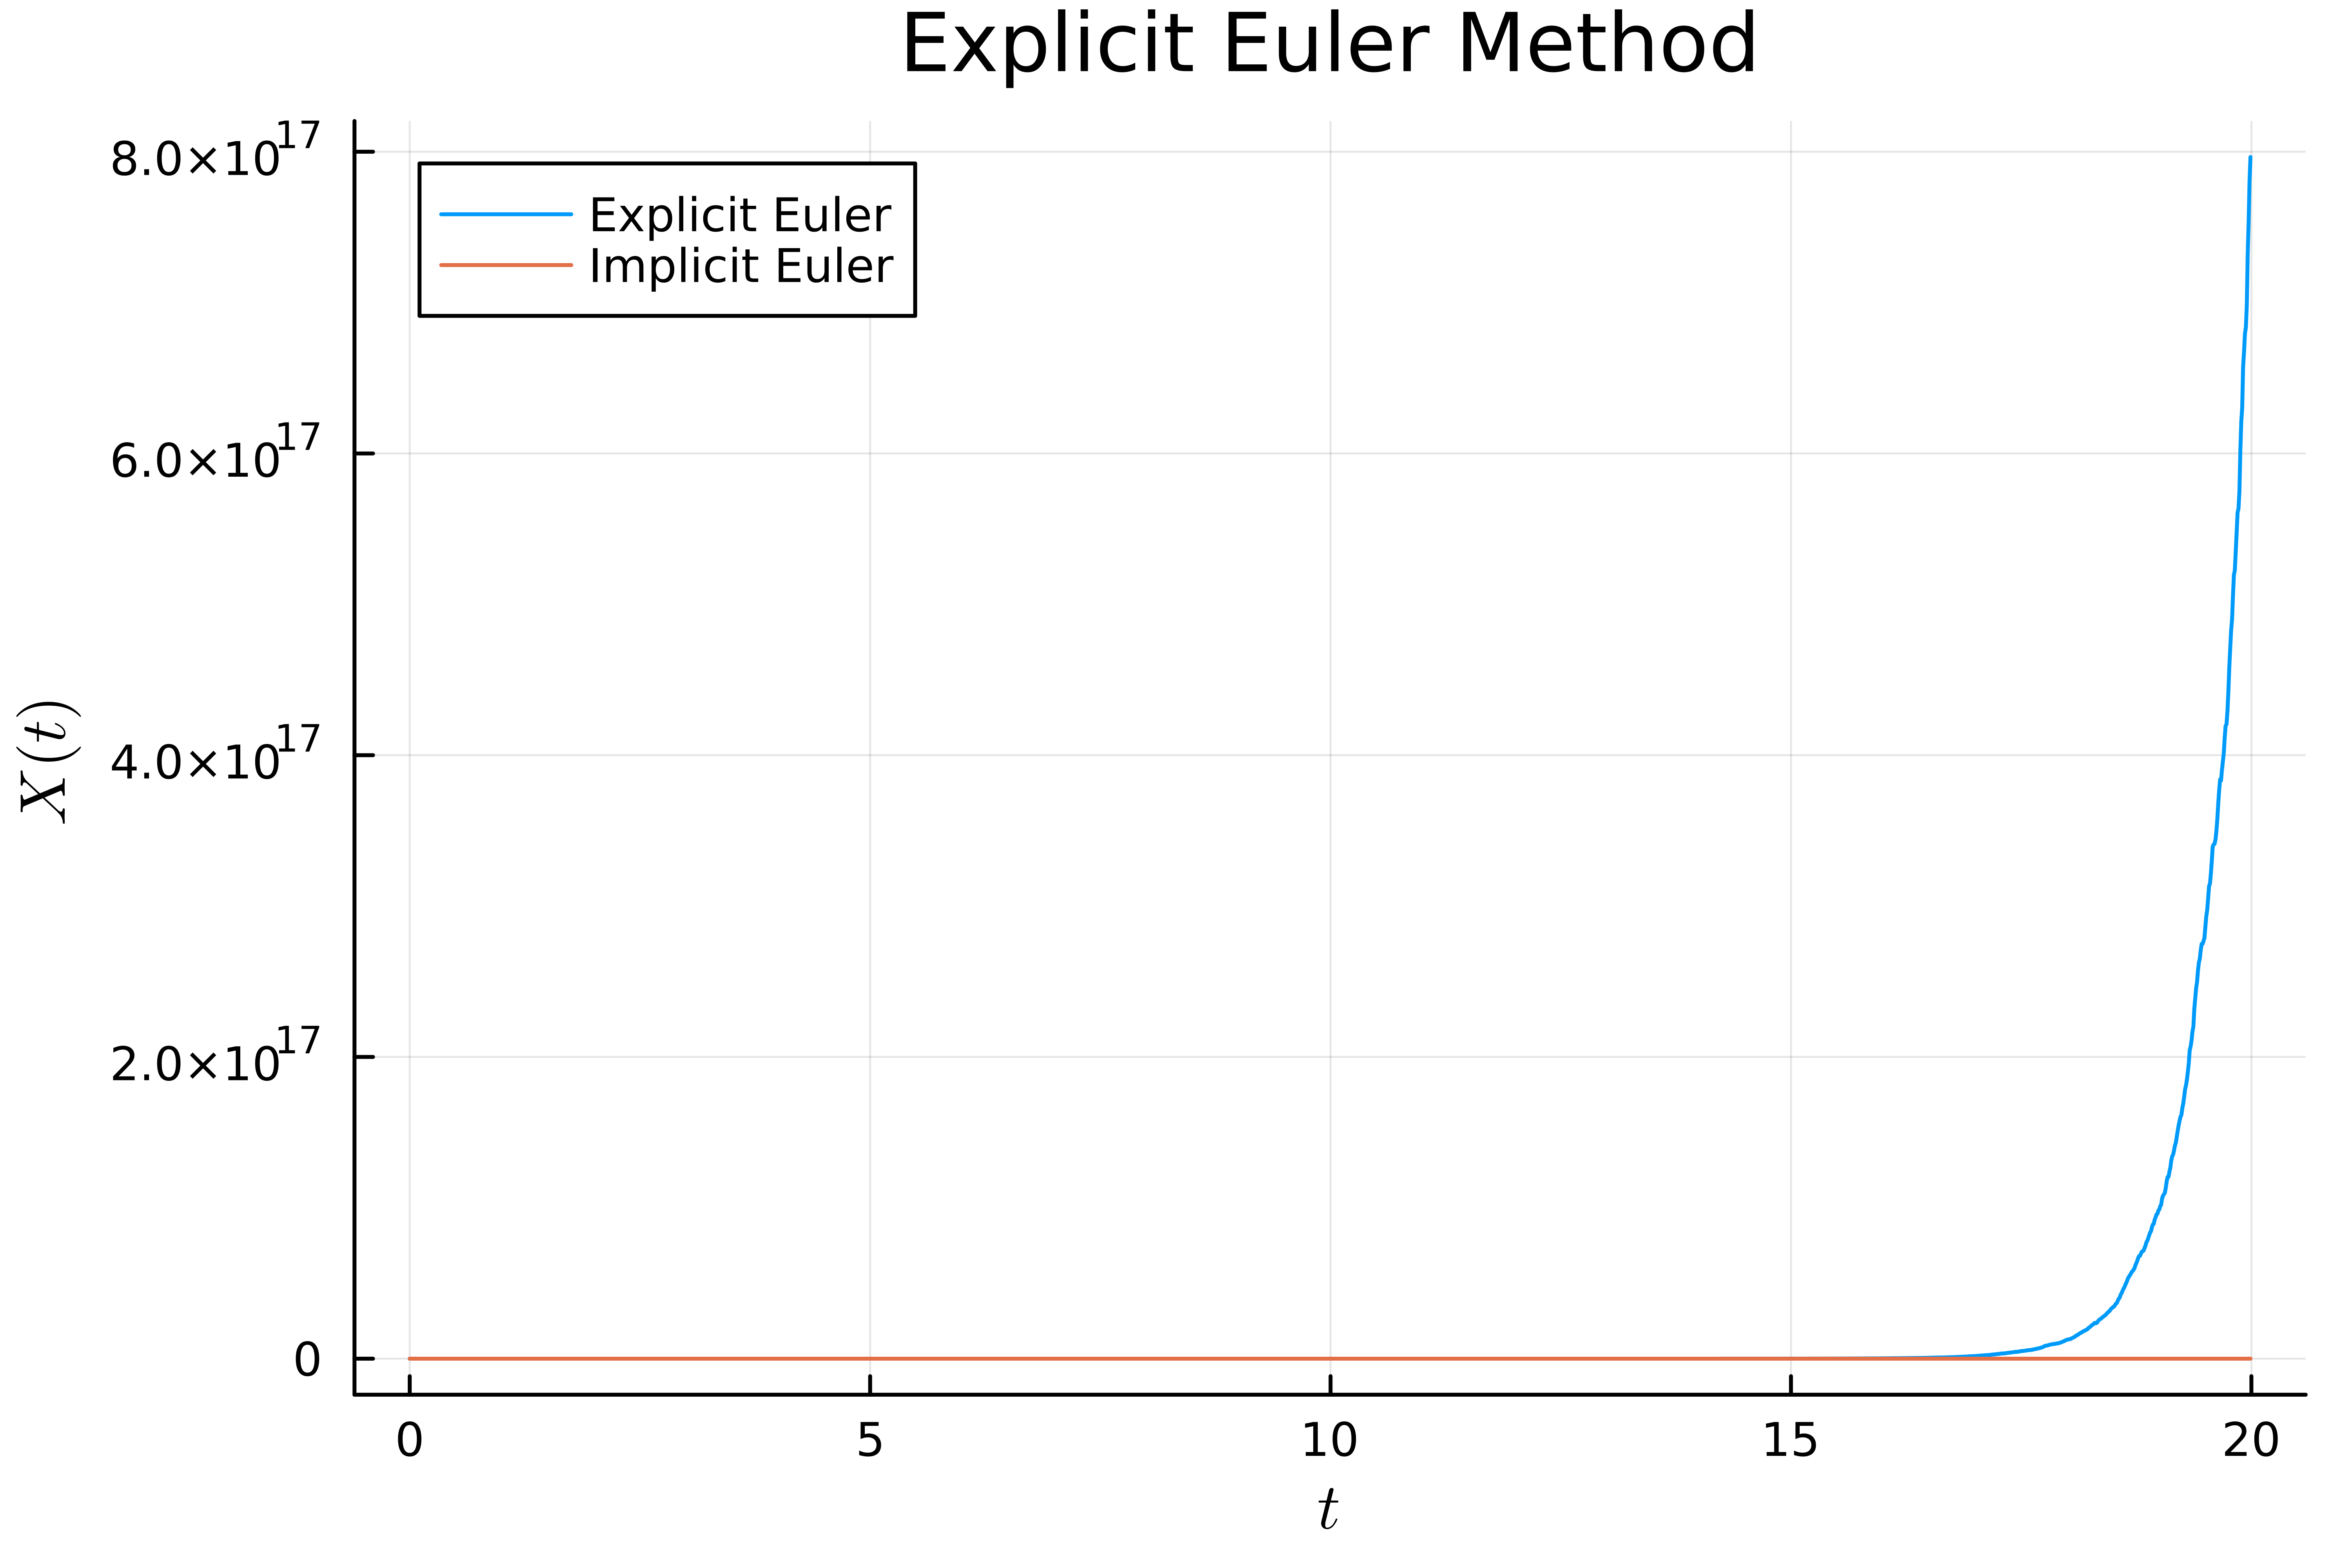
\includegraphics[scale=0.05]{imgs/4explicit_euler.png}
    \caption{Explicit Euler}
    \label{fig:expliciteuler}
\end{figure}

\begin{figure}[H]
    \centering
    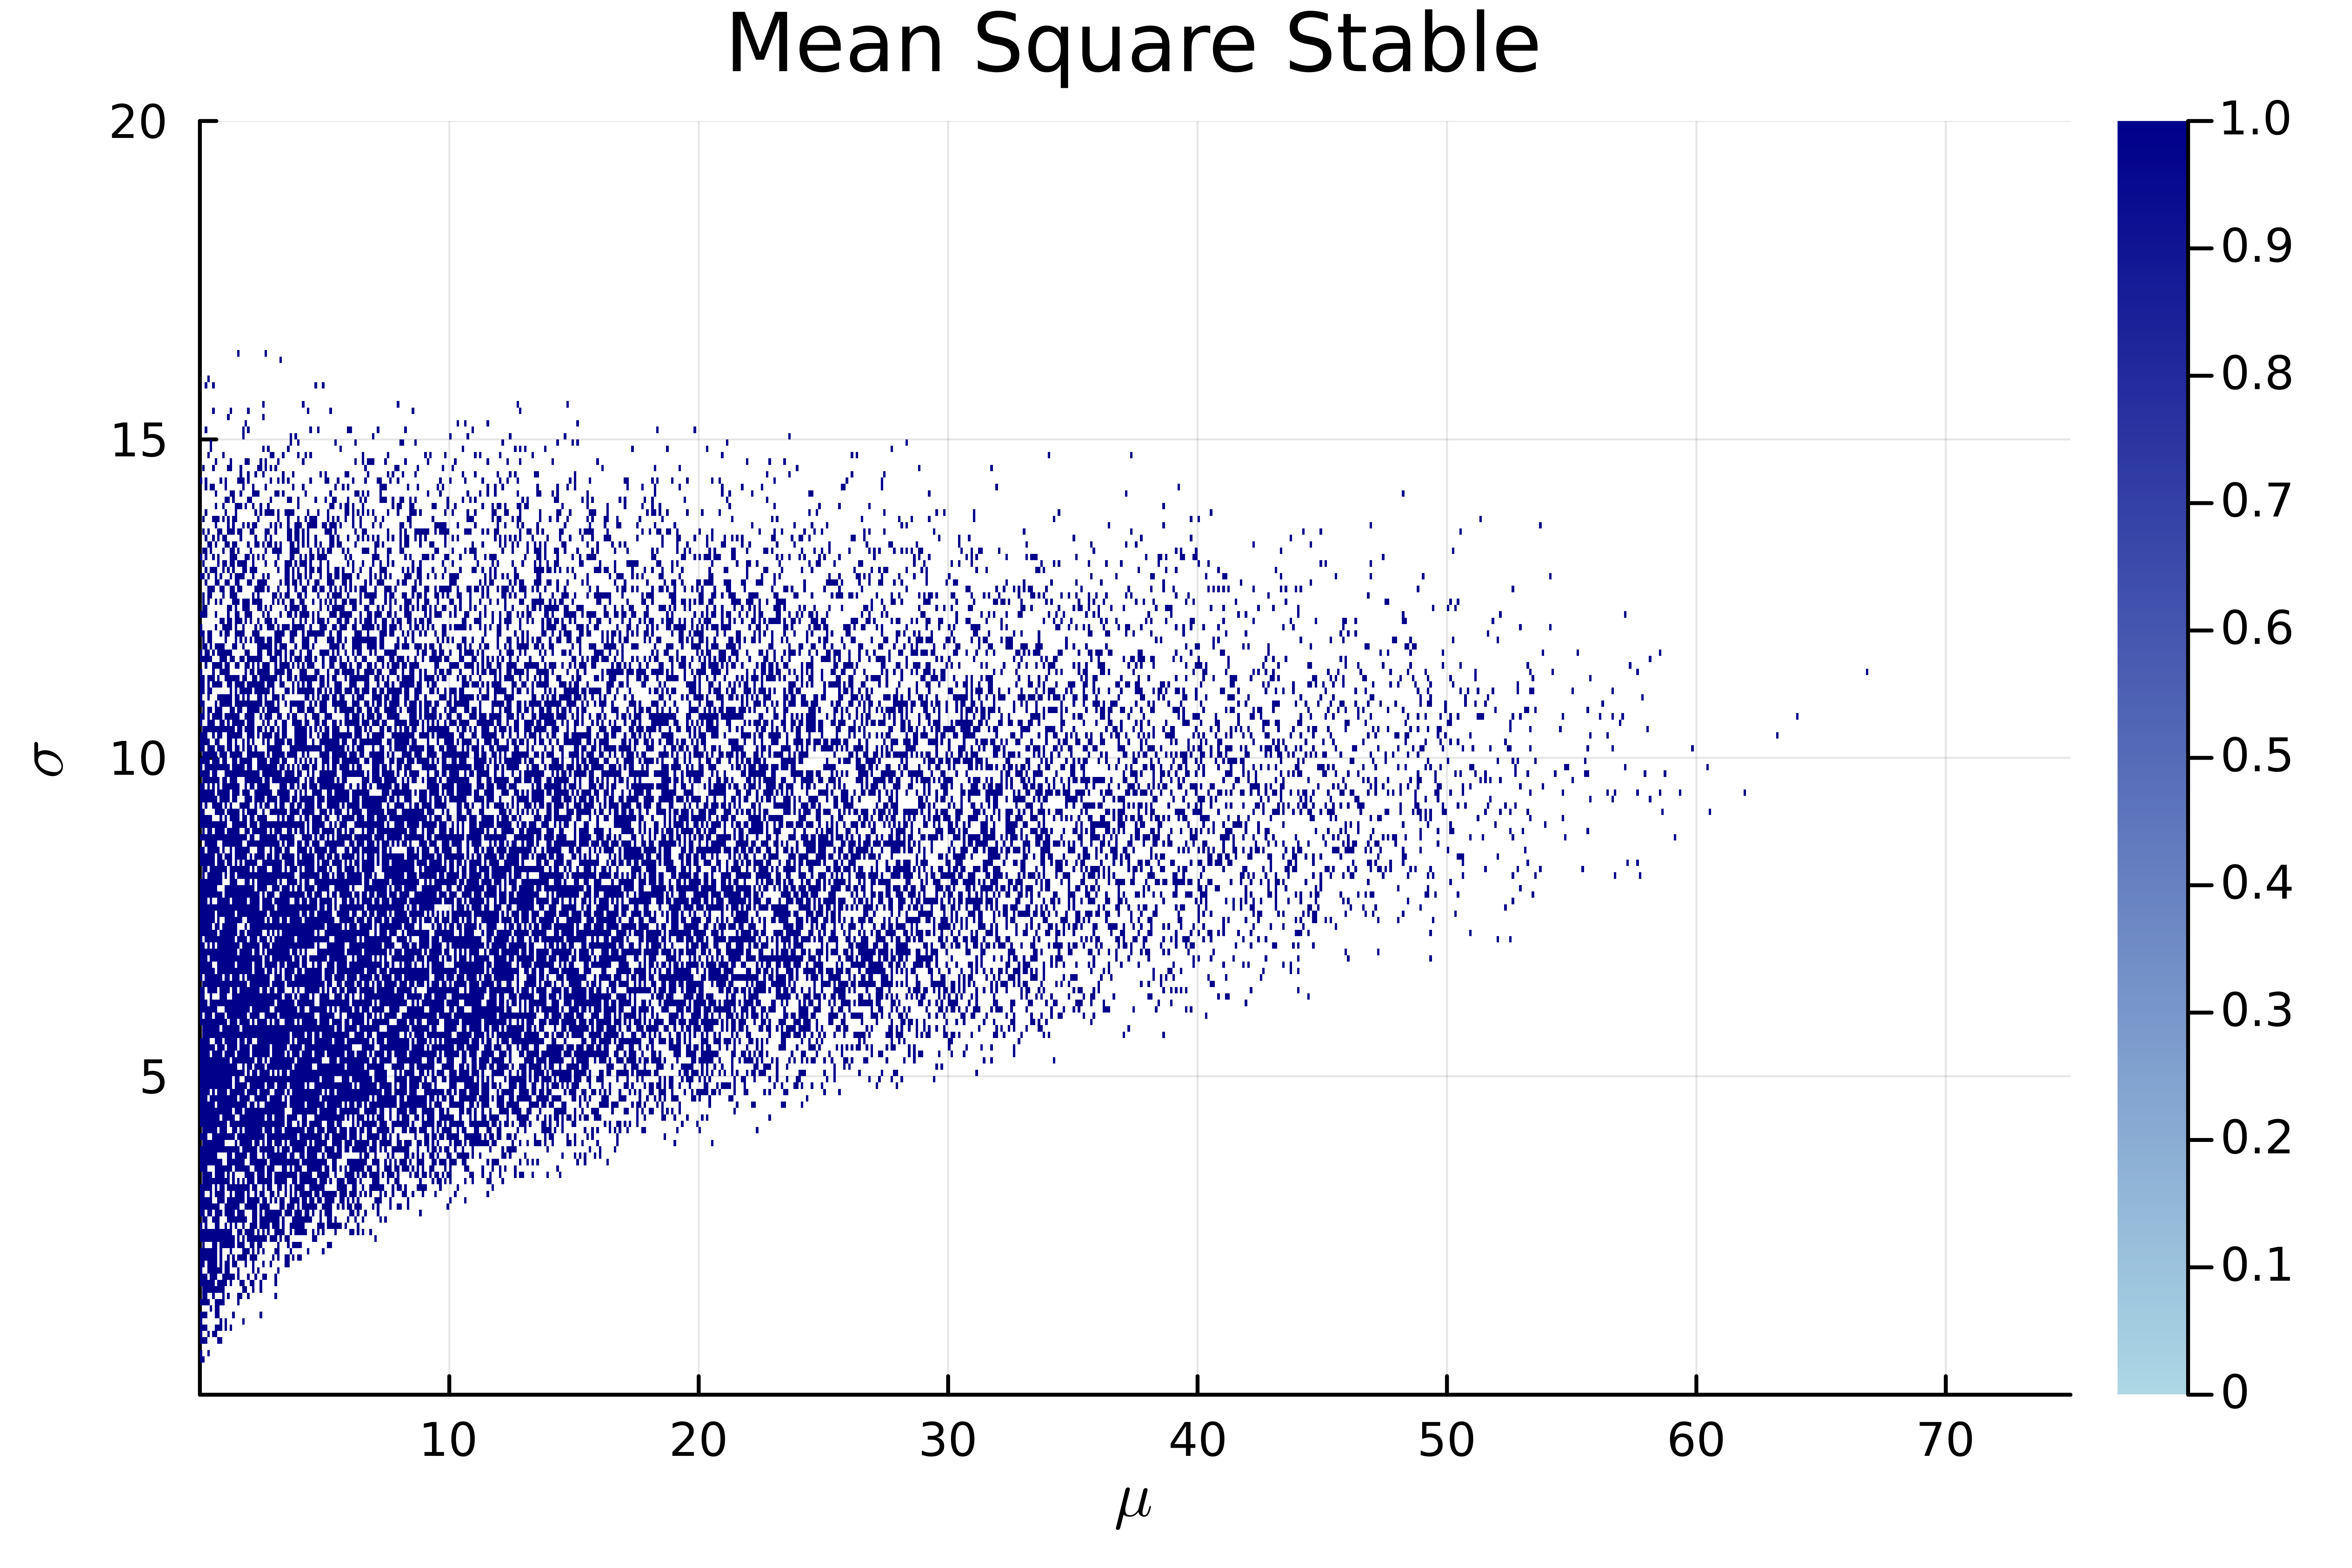
\includegraphics[scale=0.05]{imgs/4mean_square_stable.png}
    \caption{Mean Square Stable Values}
    \label{fig:meansq}
\end{figure}



\section*{Question 5}

\begin{figure}[H]
    \centering
    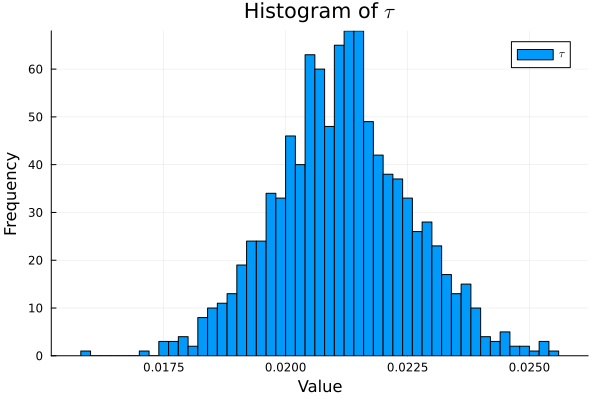
\includegraphics[scale=0.6]{imgs/5.png}
    \caption{5}
    \label{fig:5}
\end{figure}
\end{document}